\documentclass[modern]{aastex631}

\usepackage{amsmath}

\begin{document}

\title{A Practical Line Cleaner for Narrow Lines in Gravitational Wave Data}

\author[0000-0003-1540-8562]{Will M. Farr}
\email{will.farr@stonybrook.edu}
\email{wfarr@flatironinstitute.org}
\affiliation{Department of Physics and Astronomy, Stony Brook University, Stony Brook, NY 11794, USA}
\affiliation{Center for Computational Astrophysics, Flatiron Institute, New York, NY 10010, USA}

\begin{abstract}
    I present a tool, \texttt{linecleaner}, for fitting and regressing
    narrow-band lines from timeseries data such as appear frequently in
    gravitational wave detectors.  Residuals produced by this tool can be passed
    onward to analyses that will benefit from removal of the (semi)coherent
    lines, as opposed to their suppression by an enhanced spectral density
    estimate around the line (a form of ``notch filter'').
\end{abstract}

\section{Theory}
\label{sec:theory}

Consider a simple harmonic oscillator driven by a stochastically-fluctuating
signal, $n(t)$,
\begin{equation}
    \ddot{x}(t) + 2\gamma\dot{x}(t) + \left( 2 \pi f_0 \right)^2 x(t) = n(t),
\end{equation}
with damping rate $\gamma$ and natural frequency $\omega_0$.  In the Fourier
domain, the solution satisfies the algebraic equation 
\begin{equation}
    -\left( 2 \pi f \right)^2 X(f) + 4 \pi i\gamma f X(f) + \left( 2 \pi f_0 \right)^2 X(f) = N(f),
\end{equation}
or
\begin{equation}
    X(f) = \frac{N(f)}{\left( 2 \pi f_0 \right)^2 - \left( 2 \pi f \right)^2 + 4 \pi i\gamma f},
\end{equation}
if we ignore the free, homogeneous solutions to the differential equation (which
anyway must damp out over timescales $\tau \gg \gamma^{-1}$).  If $n$ is
wide-sense stationary and zero-mean, then 
\begin{eqnarray}
    \left\langle N \right\rangle & = & 0, \\
    \left\langle N^*(f)N(f') \right\rangle & = &
    S_n(f) \delta(f - f'),
\end{eqnarray}
for some (positive) function $S_n$, called the power spectral density of the
noise $n$.  This implies 
\begin{eqnarray}
    \left\langle X \right\rangle & = & 0, \\
    \left\langle X^*(f)X(f') \right\rangle & = & \frac{S_n(f)}{\left(\left( 2 \pi f_0 \right)^2 - \left( 2 \pi f \right)^2\right)^2 + 16 \pi^2 \gamma^2 f^2}\delta(f - f') \equiv S_x(f) \delta\left( f - f' \right).
\end{eqnarray}
If, furthermore, $n$ is Gaussian distributed, then $x$ will be as well,
following an independent Gaussian distribution at each frequency $f$ with mean
and variance indicated above.  Many narrow-band features (lines) in
gravitational wave data can be adequately described by this model.  

Assuming $\gamma / f_0 \ll 1$ (i.e.\ that the oscillator is severely
under-damped), over short timescales $\tau$ that are longer than the natural
period associated to the solution, but short compared to the damping time, i.e.\
$f_0^{-1} \ll \tau \ll \gamma^{-1}$, the solution is sinusoidal with frequency
$f_0$.  Over longer timescales the solution oscillates at the natural frequency,
but with randomizing \emph{phase}. For some lines in present-day gravitational
wave detectors, the damping time is much longer than the analysis segments of
typical signals; in such cases, it is possible to use data from before and after
(and during) the analysis segment to \emph{infer} the phase of the line through
the analysis segment and \emph{regress} it out of the data, improving the
signal-to-noise ratio of the signal.  This is the basic idea behind the line
cleaner described in this note.

Given a stretch of data in the (discrete) Fourier domain from a total
observation time $T$, 
\begin{equation}
    D_k \simeq D\left( f = \frac{k}{T} \right) = \frac{T}{N} \sum_{n=0}^{N-1} d_n e^{-2\pi i k n / N},
\end{equation} 
and restricting our attention to a narrow range of frequencies $f_l < f < f_h$
around a line that we want to regress, it is reasonable to assume that the data
are a sum of the line and some background, continuum noise; we can assume that
the background noise power spectrum, $S_0$, is constant because the bandwidth is
narrow. Then the likelihood for the data $D$ given the line contribution $X$ is 
\begin{equation}
    p\left( D_k \mid X_k, S_0 \right) = N\left( D_k \mid X_k, \sqrt{T S_0} \right).
\end{equation}
(In words: the data are normally distributed with mean $X$ and standard
deviation $\sqrt{T S_0}$.)  It is also reasonable to assume that the
line-driving noise spectrum $S_n$ is constant over the narrow bandwith; we have
seen above that the line itself is normally distributed with mean zero and
variance $S_x(f) T$, so 
\begin{equation}
    p\left( X_k \mid S_n, f_0, \gamma \right) = N\left( X_k \mid 0, \sqrt{S_x\left(f_k \mid S_n, f_0, \gamma \right) T} \right).
\end{equation}
The product of these two normal distributions is, itself a normal distribution;
and it can be factorized in various ways \citep{Hogg2020}.  One factorization
writes it as a product of the marginal likelihood for the data given line
parameters and continuum noise,
\begin{equation}
    p\left( D_k \mid S_n, f_0, \gamma, S_0 \right) = N\left( D_k \mid 0, \sqrt{S_x\left(f_k \mid S_n, f_0, \gamma \right) T + S_0 T} \right);
\end{equation}
and the conditional posterior for the line $X_k$ given the data and parameters 
\begin{multline}
    p\left( X_k \mid D_k, S_n, f_0, \gamma, S_0 \right) \\ = N\left( X_k \mid \frac{S_x\left(f_k \mid S_n, f_0, \gamma \right) D_k}{S_x\left(f_k \mid S_n, f_0, \gamma \right) + S_0}, \sqrt{\frac{S_x\left(f_k \mid S_n, f_0, \gamma \right) S_0 T}{S_x\left(f_k \mid S_n, f_0, \gamma \right) + S_0}} \right).
\end{multline}

Applying a prior on the line and continuum parameters, and using standard
stochastic sampling techniques (MCMC, HMC, etc) allows to explore the posterior
over $S_n$, $f_0$, $\gamma$, and $S_0$ given data; for each sample, we can then
draw the line $X_k$ from the conditional posterior above.  

Subtracting a fair draw of the line from the data generates a residual sample, 
\begin{equation}
    R_k \equiv D_k - X_k,
\end{equation}
which can then be passed to downstream data analysis pipelines.  We choose to
pass onward a fair sample of the residuals instead of, say, the maximum
likelihood residuals so that the noise properties of the residuals are
un-biasedly described by the spectral density $S_0$; see Appendix
\ref{sec:oversubtract}.

\section{Implementation}

We have implemented\footnote{\url{https://github.com/farr/LineCleaner}} a model for
line cleaning as described above using Hamiltonian Monte Carlo \citep{Neal2011}
as implemented in \texttt{numpyro} \cite{bingham2019pyro,phan2019composable} to
sample over the line parameters and continuum noise level; the same model draws
the line from the conditional distribution described above at each sample of the
line parameters.  The model fitting and line subtraction for an arbitrary number
of lines in narrow bandwidth ranges supplied by the user is encapsulated in a
single function, \texttt{clean\_lines}, which returns time-domain residuals and
optionally the output of the MCMC sampling for each line.

Time domain data are tapered with an apodizing Tukey window before being
discrete Fourier transformed for the fitting in the frequency domain.  Residuals
are returned for all data \emph{outside} the tapered region.

\subsection{Fitting Considerations}

One consideration in this sort of analysis is the length of data to fit.  The
user should ensure (after tapering) there are at least several correlation times
$\tau = 1/\gamma$ of the line avaliable to fit; longer data segments will not
substantially improve the subtraction of the line (even if they will improve
knowledge of the line's parameters), because the phase of the line ``resets''
after each correlation time.  Long data segments can hurt if the data are
significantly non-stationary, since the model assumes stationarity; this can be
particularly bad if the actual physical line parameters are changing throughout
the longer data segment.  In practice, in LIGO data, the cleaner seems to work
well with between several tens and several thousands of seconds of data,
depending on the intrinsic width of the line.

The bandwidth should be chosen as narrow as possible, but wide enough to ensure
that the wings of the line have fallen well below the continuum noise level.
This is for two reasons: first, the line will only be subtracted from the data
within the chosen bandwidth, so you want to include all data where the line
could be relevant; second, you need to ensure that the model has a good estimate
of the continuum noise level.

\subsection{Example}

Here we show an example of cleaning lines at $60 \, \mathrm{Hz}$, $120 \,
\mathrm{Hz}$, and $180 \, \mathrm{Hz}$ out of data from the Hanford LIGO
observatory around the time of GW150914.  The data are available from the
Gravitational Wave Open Science Center (GWOSC)
\cite{GWOSC,GWOSC2,GW150914-GWOSC}.  We use $4096 \, \mathrm{s}$ of data sampled
at $4096 \, \mathrm{Hz}$.  The code is available in a Jupyter
notebook\footnote{\url{https://github.com/farr/LineCleaner/blob/main/LineCleaner.ipynb}}.
The full original and cleaned power spectral densities are shown in Figure
\ref{fig:cleaned-psd}, and in a narrow band around each cleaned line in Figure
\ref{fig:line-zoom}.  The line cleaner is able to remove the lines and leave a
residual consistent with the continuum noise level.

\begin{figure}
    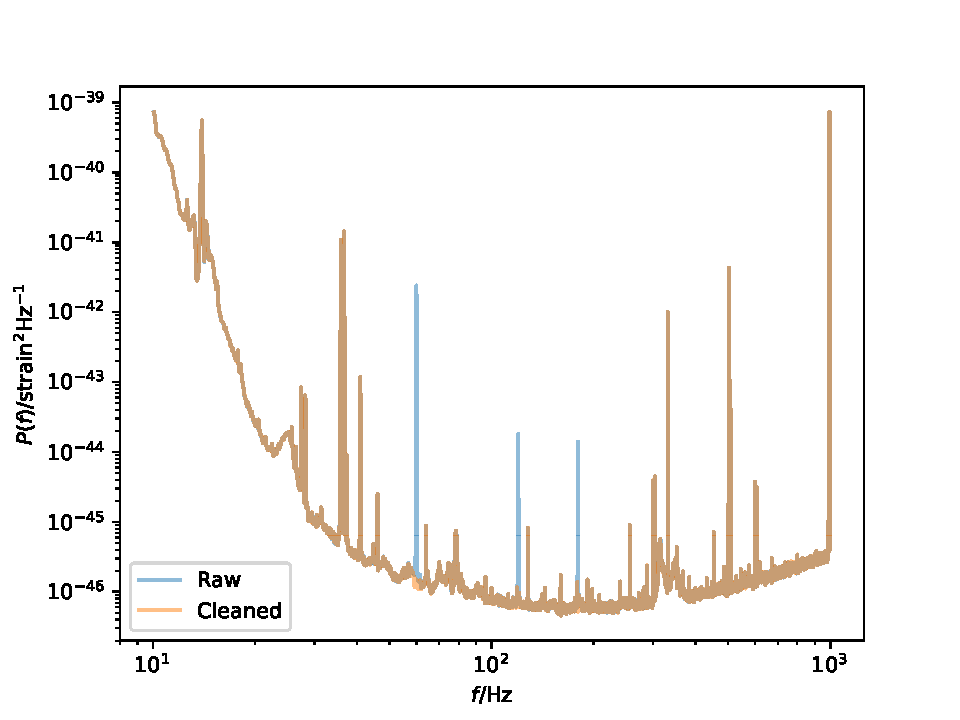
\includegraphics[width=\columnwidth]{raw-and-cleaned-psd.pdf}
    \caption{\label{fig:cleaned-psd} An example of a cleaning of data from the
    Hanford LIGO observatory around the GW150914 event
    \cite{Abbott2016,Abbott2019,GWOSC,GWOSC2,GW150914-GWOSC}.  The raw and
    cleaned data power spectral density is shown from $10 \, \mathrm{Hz}$ to $1
    \, \mathrm{kHz}$.  The lines at $60 \, \mathrm{Hz}$, $120 \, \mathrm{Hz}$,
    and $180 \, \mathrm{Hz}$ are clearly visible in the raw data, but are
    removed by the line cleaner; the cleaning used $4 \, \mathrm{Hz}$ bandwidth
    around each line.  Figure \ref{fig:line-zoom} shows a zoomed view of the
    PSDs in the vicinity of each line.}
\end{figure}

\begin{figure}
    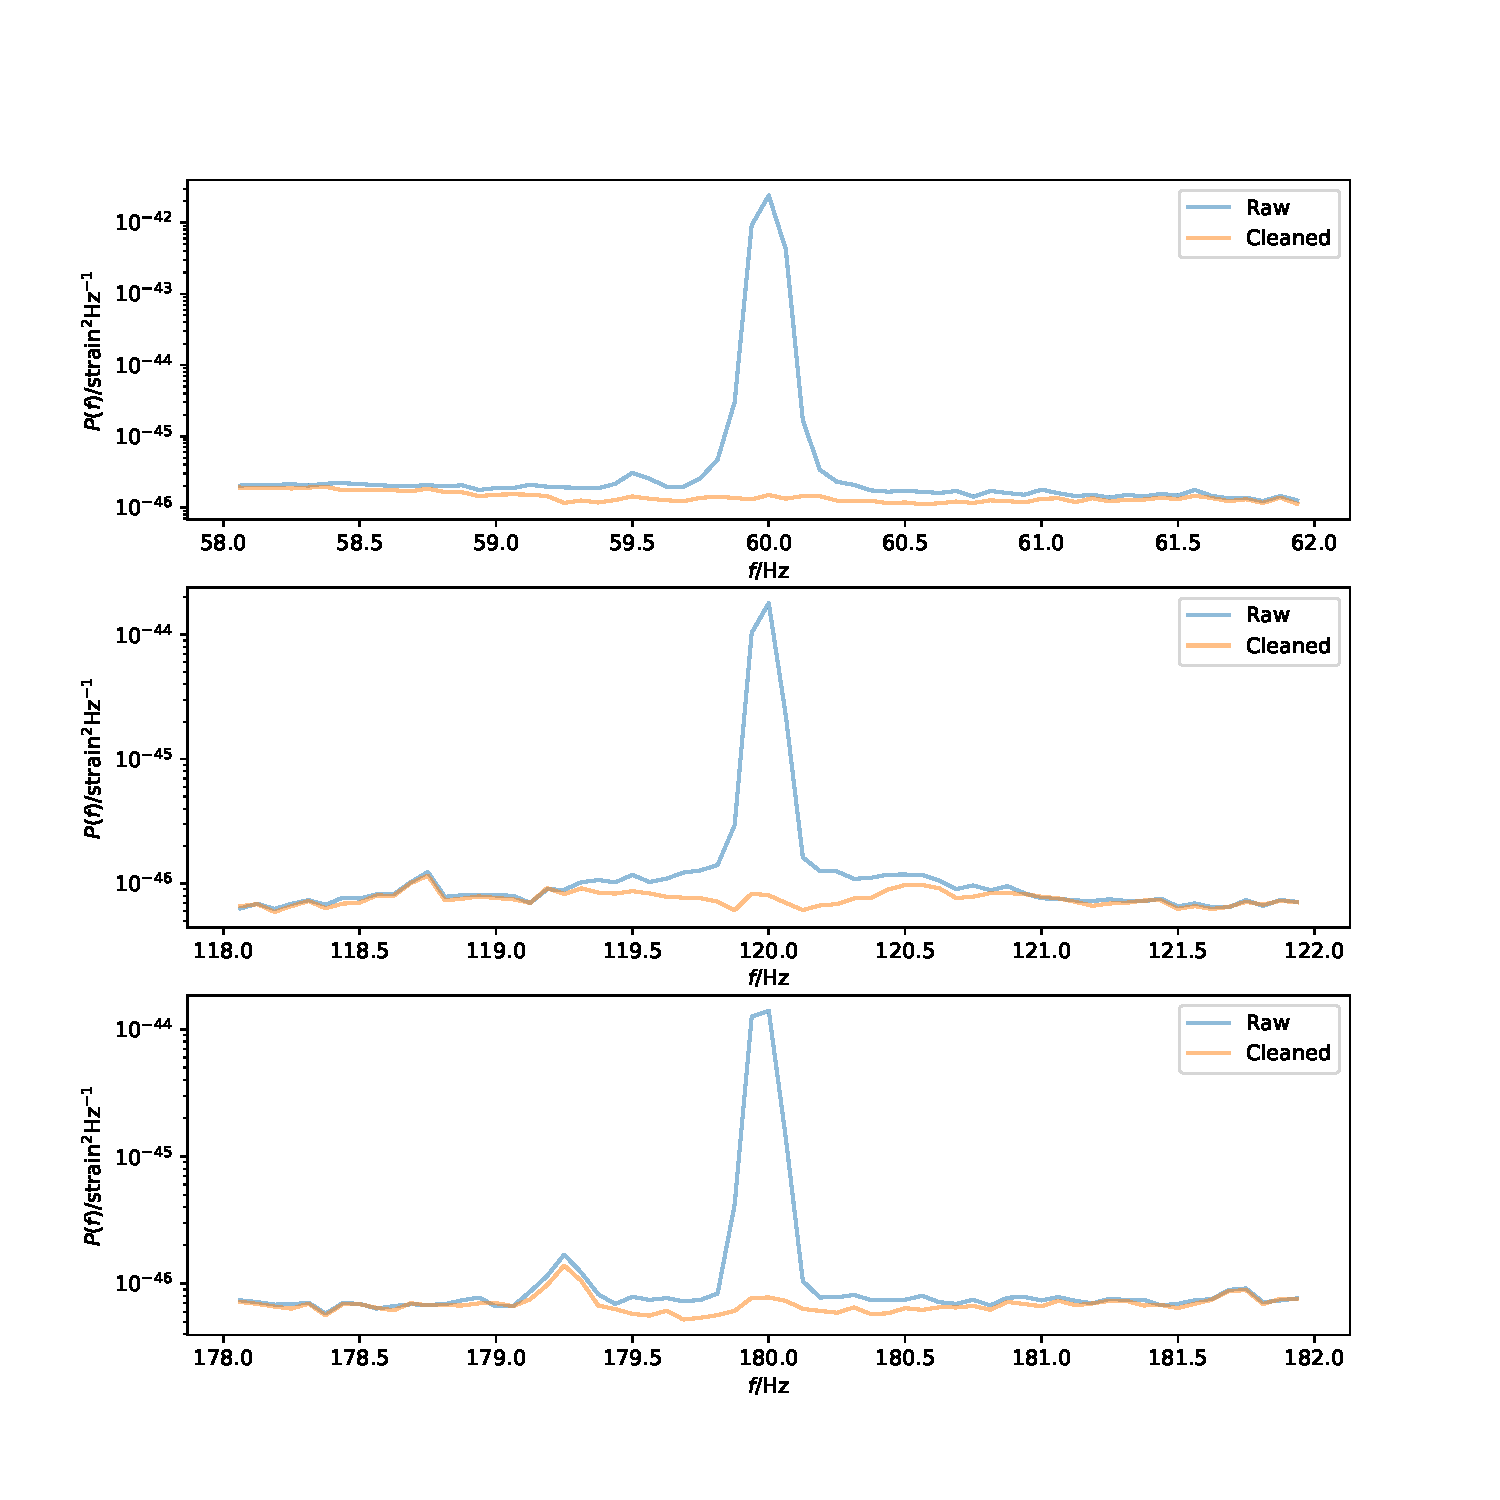
\includegraphics[width=\columnwidth]{line-zoom-in.pdf}
    \caption{\label{fig:line-zoom} A zoom-in of the power spectral densities of
    the raw and cleaned data shown in Figure \ref{fig:cleaned-psd} around the lines cleaned at .}
\end{figure}

\software{This work made use of the following software packages: \texttt{Jupyter } \citep{2007CSE.....9c..21P, kluyver2016jupyter}, \texttt{matplotlib } \citep{Hunter:2007}, \texttt{numpy } \citep{numpy}, \texttt{pandas } \citep{mckinney-proc-scipy-2010, pandas_13819579}, \texttt{python } \citep{python}, \texttt{scipy } \citep{2020SciPy-NMeth, scipy_14630489}, \texttt{ArviZ } \citep{arviz_2019, ArviZ_13854799}, \texttt{JAX } \citep{jax2018github}, \texttt{numpyro } \citep{phan2019composable, bingham2019pyro}, \texttt{tqdm } \citep{tqdm_14231923}, and \texttt{xarray } \citep{hoyer2017xarray, xarray_14777280}.  Software citation information aggregated using \texttt{\href{https://www.tomwagg.com/software-citation-station/}{The Software Citation Station}} \citep{software-citation-station-paper, software-citation-station-zenodo}.}

\appendix

\section{Avoiding Over-Subtraction}
\label{sec:oversubtract}

As discussed in Section \ref{sec:theory}, the line cleaner algorithm subtracts a
fair draw from the posterior over the line parameters and line values, instead
of using the maximum-likelihood values for either of these quantities.  This
procedure avoids oversubtraction of the line, which is particularly important if
downstream analyses are producing, for example, a noise estimate from the
residuals.  As can be seen in Figure \ref{fig:line-zoom}, the residuals are
consistent with the continuum noise level when a fair draw is subtracted; this
would not be the case were the maximum-likelihood line used to produce the
residuals.

To motivate this choice, consider the following very simple example which nevertheless retains crucial features of the line cleaning problem.  Let us suppose that we are trying to estimate a single, scalar quantity, $x$, from data $d$ that is a sum of $x$ and some Normally distributed noise, $n \sim N(0,\sigma)$,
\begin{equation}
    d = x + n.
\end{equation}
The maximum likelihood estimate for $x$, denoted $\hat{x}$, is 
\begin{equation}
    \hat{x} = d,
\end{equation}
which leaves zero residual when subtracted from the data:
\begin{equation}
    r = d - \hat{x} = 0.
\end{equation}
On the other hand, the posterior for $x$ given $d$ is normally distributed with
mean $d$ and standard deviation $\sigma$,
\begin{equation}
    p(x \mid d) = N(x \mid d, \sigma).
\end{equation}
A fair draw from this posterior, subtracted from $d$, leaves a residual that is
also Normally distributed with mean zero and standard deviation $\sigma$, which
is exactly the correct distribution for residual noise to pass onward to
downstream analyses.  The maximum-likelihood model \emph{over-subtracts}
relative to the fair draw, producing residuals that are biased low compared to
the actual noise process in the data.  For this reason, we choose to subtract a
line estimated by a fair draw from our posterior to produce the residuals that
we pass onward.

\bibliographystyle{aasjournal}
\bibliography{linecleaner}

\end{document}